% !TEX root = 0000.tex
% Capítulo 2: Physics-Informed Neural Networks
% Contenido tomado de main_2.tex (líneas 1570-2617) sin cambios de texto.

% El texto está en inglés: reglas de corte de palabra del inglés
\begin{hyphenrules}{english}

\chapter{Physics-Informed Neural Networks - PINN}\label{ch:pinns}

Solving partial differential equations has traditionally relied on classical numerical methods, most
prominently the finite difference method (FDM), the finite element method (FEM), and the finite volume
method (FVM). Because analytical solutions are not available for most real-world problems, these
approaches discretize the spatial and temporal domains into meshes or grids, replacing continuous
derivatives with algebraic operators and often requiring simplified approximations. Although these
methods allow one to estimate the prediction accuracy, or to improve convergence by increasing the
mesh density, the number of basis functions, or the simulation time, they are typically computationally
expensive and present technical difficulties in their implementation and adaptation to a specific
problem, requiring deep knowledge of the particular system to determine whether the technique is
suitable.

This chapter presents physics-informed neural networks (PINNs) as an alternative. It is organized
following the three sources of error of a PINN (approximation, generalization and optimization):
Section~\ref{sec:pinn-background} places PINNs among the numerical methods; Section~\ref{sec:pinn-formulation}
gives the formal definition; Section~\ref{sec:pinn-theory} collects the modern theory that bounds each source
of error, including an energy estimate for the Klein--Gordon equation; Sections~\ref{sec:optimization} and \ref{sec:gradient-pathologies}
analyze the optimization problem and its pathologies; and
Sections~\ref{sec:training-strategies}, \ref{sec:representation}, \ref{sec:architectures} and \ref{sec:mabur} present the training
strategies and architectures that are compared in Chapter~\ref{ch:experiments}, ending with our proposal,
MABUR-PINN.

% =====================================================================
\section{From Classical Numerical Methods to Neural Networks}\label{sec:pinn-background}
% =====================================================================

Table~\ref{tab:classical-methods} summarizes the classical methods. All of them are well understood and,
for problems of moderate size and simple geometry, they remain the reference. However, classical
mesh-based methods face severe limitations when addressing real-world problems:
\begin{enumerate}
  \item \textbf{Curse of dimensionality.} The high dimensionality of the domain implies an exponential
    growth of the computational and memory cost.
  \item \textbf{Complex mesh generation.} For geometrically complex, irregular or time-evolving domains,
    building and refining the computational mesh is technically difficult and costly.
  \item \textbf{Data.} Measurements are not incorporated in a natural way into classical numerical
    methods.
  \item \textbf{High data cost of pure networks.} On the other side, purely data-driven neural
    networks require large amounts of labeled data.
\end{enumerate}
This rigidity contrasts with the flexibility of emerging deep learning paradigms, such as
physics-informed neural networks (PINNs), which can combine data with physical knowledge expressed as
PDEs and are conceptually general and independent of the complexity of the underlying equations.

\begin{table}[htbp]
  \centering
  \caption{Classical numerical methods for PDEs.}
  \label{tab:classical-methods}
  \small
  \begin{tabularx}{\linewidth}{@{}lXX@{}}
    \toprule
    Method & Representative authors & Key idea \\
    \midrule
    Finite differences (FDM) & Causon and Mingham~\cite{causon2010}; Strikwerda~\cite{strikwerda2004} &
      Replaces derivatives by algebraic differences on a space--time grid. \\
    Finite elements (FEM) & Reddy~\cite{reddy2019}; Zienkiewicz et al.~\cite{zienkiewicz2013} &
      Subdivides the domain and solves the weak form with piecewise polynomials. \\
    Finite volumes (FVM) & Eymard et al.~\cite{eymard2000}; Moukalled et al.~\cite{moukalled2016} &
      Conserves physical fluxes in discrete control volumes. \\
    Spectral methods & Hesthaven et al.~\cite{hesthaven2007}; Shen et al.~\cite{shen2011} &
      Projects the solution onto global bases: Chebyshev, Legendre or Fourier. \\
    \bottomrule
  \end{tabularx}
\end{table}

\paragraph{Mathematical foundations and first ideas.}
The use of neural networks as numerical methods rests on the universal approximation theorems.
Cybenko~\cite{cybenko1989} and Hornik et al.~\cite{hornik1989} proved that a multilayer perceptron (MLP) with a single
hidden layer and sigmoidal activation functions can approximate any continuous function on a compact
set, and Leshno et al.~\cite{leshno1993} extended the result to any non-polynomial, locally bounded activation.
Dissanayake and Phan-Thien~\cite{dissanayake1994} proposed, very early, a neural network to approximate the solution of a PDE
by minimizing its residual, and Raissi et al.~\cite{raissi2017a,raissi2017b,raissi2019} structured the modern
framework of PINNs for forward and inverse problems. Since then, many variants have been proposed;
Table~\ref{tab:pinn-variants} groups the main ones that are relevant for this thesis.

\begin{table}[htbp]
  \centering
  \caption{Main advances and variants in the field of PINNs.}
  \label{tab:pinn-variants}
  \small
  \begin{tabularx}{\linewidth}{@{}llXX@{}}
    \toprule
    Category & Variant & Authors & Key idea \\
    \midrule
    Loss weighting & LRA / GradNorm & Wang et al.~\cite{wang2021gradient} & Balancing based on the norm of the gradients. \\
    Loss weighting & NTK weights & Wang et al.~\cite{wang2022ntk} & Calibrates weights via the neural tangent kernel. \\
    Adaptive sampling & RAR & Lu et al.~\cite{lu2021deepxde}; Wu et al.~\cite{wu2023sampling} & Adds points in zones of high residual. \\
    Architecture & LAAF / GAAF & Jagtap et al.~\cite{jagtap2020a,jagtap2020b} & Local and global adaptive activations. \\
    Architecture & Random Fourier features & Tancik et al.~\cite{tancik2020}; Wang et al.~\cite{wang2021eigenvector} & Overcomes the spectral bias at high frequencies. \\
    Architecture & RWF, modified MLP & Wang et al.~\cite{wang2022rwf,wang2023expert} & Improves representation in nonlinear problems. \\
    Architecture & SIREN & Sitzmann et al.~\cite{sitzmann2020} & Periodic sine activations. \\
    Variational & VPINNs / hp-VPINNs & Kharazmi et al.~\cite{kharazmi2019,kharazmi2021} & Polynomial test functions inspired by hp-FEM. \\
    Variational & wPINNs & De Ryck et al.~\cite{deryck2024wpinn} & Entropy solutions of hyperbolic conservation laws. \\
    Operator learning & DeepONet / FNO & Lu et al.~\cite{lu2021deeponet}; Li et al.~\cite{li2021fno} & Learns operators between function spaces. \\
    Geometric optimization & Preconditioning & De Ryck et al.~\cite{deryck2024operator} & Conditioning of the differential operator. \\
    RKHS kernels & ANaGRAM / AMStraMGRAM & Schwencke and Furtlehner~\cite{schwencke2025anagram} and Schwencke et al.~\cite{schwencke2025amstram} & The empirical natural gradient is related to the Green's function in an RKHS. \\
    \bottomrule
  \end{tabularx}
\end{table}

To address the limitations above, PINNs have emerged as a mesh-free, nonlinear parametric numerical
method \cite{raissi2019}. The fundamental premise is to use a nonlinear model, such as an MLP, to
capture both the linear and the nonlinear dynamics. Instead of discretizing the domain into a mesh,
PINNs substitute the exact solution $u(\mathbf{x},t)$ with a parametric approximator $u_\theta(\mathbf{x},t)$, where
$\theta\in\Theta\subset\mathbb{R}^{P}$ represents the trainable parameters of the network. Consequently, the
problem of finding the solution of the PDE is shifted into an optimization problem over the parameter
space.

% =====================================================================
\section{Formulation of Physics-Informed Neural Networks}\label{sec:pinn-formulation}
% =====================================================================

\begin{definicion}{PDE formulation.}\label{def:pde-formulation}
Let $\Omega\subset\mathbb{R}^d$ be a bounded spatial domain with smooth boundary $\partial\Omega$, and let
$T>0$. Let $\mathcal{D}$ be a differential operator that contains the time derivative of order
$\alpha\in\{1,2\}$ and a spatial operator, and let $\mathcal{B}$ be a boundary operator. We seek a
solution $u(\mathbf{x},t)$ satisfying the initial--boundary value problem
\[
  \begin{cases}
    \mathcal{D}[u](\mathbf{x},t)=f(\mathbf{x},t) & \text{in } \Omega\times(0,T),\\
    u(\mathbf{x},0)=g_0(\mathbf{x}) & \text{in } \Omega,\\
    \partial_t u(\mathbf{x},0)=g_1(\mathbf{x}) & \text{in } \Omega\quad(\text{only if }\alpha=2),\\
    \mathcal{B}[u](\mathbf{x},t)=h(\mathbf{x},t) & \text{on } \partial\Omega\times(0,T).
  \end{cases}
\]
For the second-order problems of Section~\ref{subsec:hyperbolic}, the natural (weak) setting is
$u\in L^2(0,T;H^1_0(\Omega))$ with $\partial_t u\in L^2(0,T;L^2(\Omega))$, $f\in L^2(0,T;H^{-1}(\Omega))$,
$g_0\in H^1_0(\Omega)$, $g_1\in L^2(\Omega)$ and $h\in L^2(0,T;H^{1/2}(\partial\Omega))$. For the
Klein--Gordon equation, $\mathcal{D}=\partial_{tt}-\nabla^2+m^2$ \cite{qian2023}.
\end{definicion}

\begin{definicion}{Approximation to the PDE formulation.}\label{def:pde-approx}
Let $u_\theta(\mathbf{x},t)$ be a parameterized function approximator, where $\theta\in\mathbb{R}^P$ denotes the set of
learnable parameters. The objective of $u_\theta$ is to approximate and solve the PDE formulation of
Definition~\ref{def:pde-formulation}.
\end{definicion}

The existence theorems for elliptic, parabolic and hyperbolic PDEs of Section~\ref{sec:second-order} establish
that solutions can be approximated using basis functions through projections (Galerkin) or collocation
methods. Definition~\ref{def:pinn} extends this classical framework by replacing the fixed set of basis functions
with a parameterized global function approximator $u_\theta$, whose parameters are learned directly from
the governing equations.

\begin{definicion}{Physics-informed neural network as approximator to the PDE formulation.}\label{def:pinn}
Let $\Omega\subset\mathbb{R}^d$ be a bounded spatial domain with boundary $\partial\Omega$, and let $[0,T]$ be
the time interval. A physics-informed neural network (PINN) is a global, parameterized function
approximator $u_\theta:\Omega\times[0,T]\to\mathbb{R}^{m}$, represented by a neural network, usually a
multilayer perceptron (MLP) with an element-wise activation function $\sigma:\mathbb{R}\to\mathbb{R}$. The network is
defined by the parameters $W^{[l]}\in\mathbb{R}^{n_l\times n_{l-1}}$ and $\mathbf{b}^{[l]}\in\mathbb{R}^{n_l}$,
$l=1,\dots,L$, where $L$ is the total number of layers. The forward propagation is given by
\cite{goodfellow2016}
\[
  \mathbf{a}^{[0]}=(\mathbf{x},t)\in\mathbb{R}^{d+1},\qquad
  \mathbf{z}^{[l]}=W^{[l]}\mathbf{a}^{[l-1]}+\mathbf{b}^{[l]},\qquad
  \mathbf{a}^{[l]}=\sigma(\mathbf{z}^{[l]}),
\]
with a linear last layer, and the output of the network is $u_\theta(\mathbf{x},t)=\mathbf{a}^{[L]}\in\mathbb{R}^m$. The
set of all learnable parameters is $\theta=\{W^{[l]},\mathbf{b}^{[l]}\}_{l=1}^{L}\in\mathbb{R}^{P}$, where
$P=\sum_{l=1}^{L}(n_ln_{l-1}+n_l)$ with $n_0=d+1$. It is found by solving a minimization problem for the
PINN loss function, which is built from the residuals of the PDE and of the initial and boundary data:
\[
  \Loss(\theta;\T)=\Loss_{\mathrm{data}}(\theta)+\Loss_f(\theta)
  =\Loss_{bc}(\theta;\T_{bc})+\Loss_{ic}(\theta;\T_{ic})+\Loss_f(\theta;\T_f),
\]
where the individual loss terms $\Loss_{bc}$, $\Loss_{ic}$, $\Loss_f$ correspond to the boundary
condition, the initial condition and the PDE, respectively, and $\T_f$, $\T_{bc}$, $\T_{ic}$ are the
corresponding sets of collocation points. The term $\Loss_{ic}$ can be divided into the initial
position $\Loss_{icp}$ and the initial velocity $\Loss_{icv}$.
\end{definicion}

The cost functions are defined through their residuals as follows:
\begin{align}
  \Loss_f(\theta;\T_f)&=\frac{1}{\abs{\T_f}}\sum_{(\mathbf{x},t)\in\T_f}\abs{R_{\mathrm{PDE}}(\mathbf{x},t;\theta)}^2,\label{eq:loss-f}\\
  \Loss_{icp}(\theta;\T_{ic})&=\frac{1}{\abs{\T_{ic}}}\sum_{\mathbf{x}\in\T_{ic}}\abs{R_{ic0}(\mathbf{x};\theta)}^2,\label{eq:loss-icp}\\
  \Loss_{icv}(\theta;\T_{ic})&=\frac{1}{\abs{\T_{ic}}}\sum_{\mathbf{x}\in\T_{ic}}\abs{R_{ic1}(\mathbf{x};\theta)}^2,\label{eq:loss-icv}\\
  \Loss_{bc}(\theta;\T_{bc})&=\frac{1}{\abs{\T_{bc}}}\sum_{(\mathbf{x},t)\in\T_{bc}}\abs{R_{bc}(\mathbf{x},t;\theta)}^2,\label{eq:loss-bc}
\end{align}
and the residuals are defined as
\begin{align}
  R_{\mathrm{PDE}}(\mathbf{x},t;\theta)&=\mathcal{D}[u_\theta](\mathbf{x},t)-f(\mathbf{x},t), \label{eq:res-pde}\\
  R_{bc}(\mathbf{x},t;\theta)&=\mathcal{B}[u_\theta](\mathbf{x},t)-h(\mathbf{x},t), \label{eq:res-bc}\\
  R_{ic0}(\mathbf{x};\theta)&=u_\theta(\mathbf{x},0)-g_0(\mathbf{x}), \label{eq:res-ic0}\\
  R_{ic1}(\mathbf{x};\theta)&=\partial_t u_\theta(\mathbf{x},0)-g_1(\mathbf{x}). \label{eq:res-ic1}
\end{align}
Here $\mathcal{D}$ is the differential operator governing the PDE, $\mathcal{B}$ defines the boundary
conditions $\mathcal{B}[u](\mathbf{x},t)=h(\mathbf{x},t)$, and $u(\mathbf{x},0)=g_0(\mathbf{x})$ and $\partial_t u(\mathbf{x},0)=g_1(\mathbf{x})$ are the
initial conditions for position and velocity. The derivatives of $u_\theta$ with respect to $\mathbf{x}$ and $t$
are computed exactly by automatic differentiation. Each sum is a Monte Carlo (or quadrature)
approximation of the corresponding $L^2$ norm, for example
\[
  \Loss_f\approx\abs{\Omega\times(0,T)}^{-1}\norm{R_{\mathrm{PDE}}}_{L^2(\Omega\times(0,T))}^2.
\]
When
experimental data are available, a data term of the same form is added to the cost function. The optimal
parameters are found by solving the minimization problem
\begin{equation}
  \theta^{*}(\T)=\argmin_{\theta\in\Theta}\Loss(\theta;\T).
  \label{eq:pinn-argmin}
\end{equation}

\paragraph{Three errors.}
A good approximation is one in which the residual is as close to zero as possible, but a small loss is
not the same as a small error. Following De Ryck and Mishra~\cite{deryck2024acta}, we distinguish:
\begin{itemize}
  \item the \emph{total error} $\mathcal{E}(\theta)=\norm{u-u_\theta}_X$, typically with $X=L^2(\Omega)$;
  \item the \emph{generalization error} $\mathcal{E}_G(\theta)=\norm{R_{\mathrm{PDE}}}_{L^2}+\dots$, the
    continuous physics-informed residual (all the terms of the loss measured in their continuous norms);
  \item the \emph{training error} $\mathcal{E}_T(\theta;\T)=\sqrt{\Loss(\theta;\T)}$, the discretized
    residual that the optimizer actually sees.
\end{itemize}
In the language of statistical learning (Figure~\ref{fig:shin-errors}), the optimization error is the
difference between the network that we have trained and the best network that the optimizer could find
in the chosen class; the approximation error is the difference between the exact function (or the
reference numerical method) and the best network of the class; and the estimation (generalization) error
is the error associated with points of the domain that were not part of the training. When we speak of
these three errors, we assume that there exists an ideal network, theoretically or empirically better
trained, with respect to which our approximation is compared.

\begin{figure}[htbp]
  \centering
  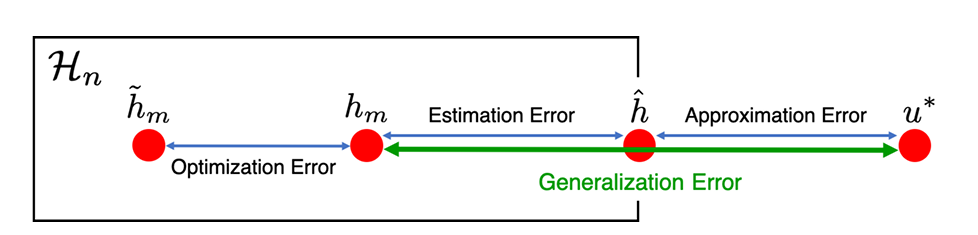
\includegraphics[width=0.75\linewidth]{shin_error_diagram.png}
  \caption[Errors that appear when training a PINN]{Diagram of the different errors that appear when training a PINN: optimization,
  estimation and approximation errors.}
  \label{fig:shin-errors}
  \fuente{Shin et al.~\cite{shin2020convergence}.}
\end{figure}
\verificar{permission / ``adapted from'' for the reproduced figure}

% =====================================================================
\section{Modern Theory of PINNs}\label{sec:pinn-theory}
% =====================================================================

This section collects the results that bound each of the three errors. We do not prove them; the goal
is to understand what each one says about our experiments. The theorem numbers refer to the original
works.\verificar{theorem/lemma numbers against the published versions}

% ---------------------------------------------------------------------
\subsection{Error Decomposition}

\begin{teorema}{Error decomposition \cite[Lemma~3.1 and Eq.~3.11]{deryck2022generic,deryck2024acta}.}\label{thm:error-decomp}
Suppose that the PDE is stable in the sense that $\norm{u-u_\theta}_X\le C\,\mathcal{E}_G(\theta)^{\alpha}$
for some $C,\alpha>0$, and let $\hat\theta$ be the parameter of the ideal model. Then the total error
$\mathcal{E}^{*}=\norm{u-u_{\theta^{*}(\T)}}_X$ satisfies
\[
  \mathcal{E}^{*}\le C\Big(\underbrace{\mathcal{E}_G(\hat\theta)}_{\text{approximation}}
  +\underbrace{2\sup_{\theta\in\Theta}\abs{\mathcal{E}_T(\theta;\T)-\mathcal{E}_G(\theta)}}_{\text{generalization gap}}
  +\underbrace{\mathcal{E}_T(\theta^{*}(\T);\T)-\mathcal{E}_T(\hat\theta;\T)}_{\text{optimization}}\Big)^{\alpha}.
\]
\end{teorema}

The stability hypothesis is exactly where the PDE theory of Chapter~\ref{ch:pdes} enters: for elliptic and
parabolic problems it follows from coercivity and the maximum principle; for hyperbolic problems it
follows from energy estimates (Section~\ref{subsec:energy-estimate}).

% ---------------------------------------------------------------------
\subsection{Approximation Error}

\begin{teorema}{Approximation with $\tanh$ networks \cite[Theorem~4.4]{deryck2021tanh}.}\label{thm:tanh-approx}
Let $\Omega=[0,1]^d$. For every $N\in\mathbb{N}$ and every $f\in W^{s,\infty}(\Omega)$ there exists a network
with $\tanh$ activation, two hidden layers and width $N$, $\hat u$, such that for all $0\le k<s$
\[
  \norm{f-\hat u}_{W^{k,\infty}(\Omega)}\le C\big(\ln(cN)\big)^{k}N^{-(s-k)/d}.
\]
\end{teorema}

\emph{Consequence.} The network approximates not only $f$ but also its derivatives up to order $k$, which
are the ones demanded by the operator $\mathcal{D}$. The rate, however, deteriorates with the dimension
$d$.

\begin{teorema}{Sobolev--Barron approximation \cite[Theorem~4.33]{deryck2024acta}.}\label{thm:barron}
Let $\sigma$ be smooth with $C_1:=\max_{m\le\ell}\norm{\sigma^{(m)}}_{L^\infty(\mathbb{R})}<\infty$. If $f$
belongs to the spectral Barron space $\mathcal{B}^{R}_{1}(\Omega)$ (index 1, radius $R\ge1$), then for
every width $k\in\mathbb{N}$ there exists a shallow network
$u_k(\mathbf{x})=\frac1k\sum_{i=1}^{k}a_i\sigma(\mathbf{w}_i^{\top}\mathbf{x}+b_i)$ with
$(a_i,\mathbf{w}_i,b_i)\in\mathbb{R}\times B^d_R\times\mathbb{R}$ such that
\[
  \norm{u_k-f}_{H^{\ell}_{\mu}(\Omega)}\le\frac{2C_1\big(R\sqrt{ed}\big)^{\ell}\norm{f}_{\mathcal{B}^R_1(\Omega)}}{\sqrt{k}}.
\]
\end{teorema}

The rate $k^{-1/2}$ is independent of $d$: in the Sobolev--Barron regime the network overcomes the
curse of dimensionality. Notice that the activation function only enters through the constant $C_1$,
the maximum of its derivatives up to the order $\ell$ of the PDE. We will use this observation to
analyze our adaptive activations in Section~\ref{sec:mabur}.

% ---------------------------------------------------------------------
\subsection{Generalization Gap}

\begin{teorema}{Generalization gap \cite[Theorem~6.2]{deryck2022kolmogorov,beck2022}.}\label{thm:generalization}
Let $\T$ consist of $N$ points drawn i.i.d.\ according to a measure $\mu$, let $\Theta=[-R,R]^{n}$ be
compact, and let $\mathfrak{L}$ be the Lipschitz constant of the map $\theta\mapsto\mathcal{E}_G(\theta)^2$.
Then
\[
  \mathbb{E}\big[\mathcal{E}_G(\theta^{*}(\T))^2\big]\le\mathbb{E}\big[\mathcal{E}_T(\theta^{*}(\T);\T)^2\big]
  +\sqrt{\frac{2c^2(n+1)}{N}\ln\Big(\frac{R\,\mathfrak{L}\sqrt{N}}{c}\Big)}.
\]
\end{teorema}

The average gap between the training and the generalization errors is of order
\[
  \mathcal{O}\Big(\frac{K_1}{\sqrt N}\ln\big(K_2\sqrt N\big)\Big).
\] For our experiments this means that the number
of collocation points must grow with the number of parameters $n$; this is one of the reasons for the
stochastic resampling of Section~\ref{subsec:sampling}, which shows the network new points at every epoch.

% ---------------------------------------------------------------------
\subsection{Optimization: Conditioning and Spectral Bias}

\begin{teorema}{Convergence in the NTK regime \cite[Theorem~7.9]{deryck2024operator}.}\label{thm:ntk-conv}
In the neural tangent kernel (NTK) regime (wide, over-parameterized networks), the number of gradient
descent steps needed to reduce the error to $\epsilon$ is
\[
  N(\epsilon)=\mathcal{O}\big(\kappa(A)\ln(1/\epsilon)\big),\qquad\kappa(A)=\frac{\lambda_{\max}(A)}{\lambda_{\min}(A)},
\]
with
$A_{ij}=\langle\mathcal{D}\varphi_i,\mathcal{D}\varphi_j\rangle_{L^2(\Omega)}+\lambda\langle\varphi_i,\varphi_j\rangle_{L^2(\partial\Omega)}$
and $\varphi_i(\mathbf{x})=\nabla_{\theta_i}u_\theta(\mathbf{x};\theta_0)$.
\end{teorema}

\begin{teorema}{Spectral bias and conditioning \cite[Theorem~7.10]{deryck2024operator}.}\label{thm:spectral-bias}
$\kappa(A)$ is governed by the condition number of the operator $\mathcal{A}\circ TT^{*}$, where
$\mathcal{A}=\mathcal{D}^{*}\mathcal{D}$ and $TT^{*}$ is the integral operator whose kernel is associated
with the architecture.
\end{teorema}

\emph{Pathology of conditioning.} Since $\mathcal{D}^{*}\mathcal{D}$ contains derivatives of twice the
order of the PDE, high frequencies make $\kappa(A)$ blow up rapidly: a Fourier mode $e^{ikx}$ is
amplified by a factor of order $k^{4}$ for a second-order operator. For the Klein--Gordon operator,
$\mathcal{D}^{*}\mathcal{D}$ multiplies the mode $e^{i(kx-\omega t)}$ by $(\omega^2-k^2-m^2)^2$, which
is why initial conditions with several wavenumbers are a hard test.

\paragraph{Spectral convergence rate.}
In the theory of Jacot et al.~\cite{jacot2018} and its extension to PINNs by Wang et al.~\cite{wang2022ntk}, it is shown
that, under an infinitesimal learning rate, the evolution in training time $\tau$ of the vector of
predictions $\mathbf{f}_\theta(\tau)$ with respect to the targets $\mathbf{Y}$ satisfies the linear ODE
\begin{equation}
  \frac{\,d\mathbf{f}_\theta(\tau)}{\,d\tau}\approx-\mathbf{K}\big(\mathbf{f}_\theta(\tau)-\mathbf{Y}\big),
  \label{eq:ntk-ode}
\end{equation}
where $\mathbf{K}$ is the NTK. Projecting the error onto the eigenvectors $\mathbf{q}_i$ of $\mathbf{K}$,
with eigenvalues $\lambda_i$, we obtain the analytical solution
\begin{equation}
  \mathbf{q}_i^{T}\big(\mathbf{f}_\theta(\tau)-\mathbf{Y}\big)=e^{-\lambda_i\tau}\,\mathbf{q}_i^{T}\big(\mathbf{f}_\theta(0)-\mathbf{Y}\big).
  \label{eq:ntk-modes}
\end{equation}
The components of the error associated with large eigenvalues (low frequencies, for standard MLPs)
are learned first, while those associated with small eigenvalues (high frequencies) are learned
exponentially slower. This is the spectral bias, and it is the counterpart, inside the optimizer, of
the parabolic decay $e^{-\lambda_k t}$ of Equation~\eqref{eq:parabolic-modes}: the network ``diffuses'' its error
mode by mode.

% ---------------------------------------------------------------------
\subsection{Regularized Loss and the Hölder Seminorm}

For linear second-order elliptic and parabolic PDEs, Shin et al.~\cite{shin2020convergence} proved that the
PINN loss with $m_r$ residual points and $m_b$ boundary points satisfies
\begin{equation}
  \mathrm{Loss}^{\mathrm{PINN}}(h;\lambda)\le C_m\cdot\mathrm{Loss}_m(h;\lambda,\hat\lambda^{R}_m)
  +C'\big(m_r^{-\alpha/d}+m_b^{-\alpha/(d-1)}\big),
  \label{eq:shin-bound}
\end{equation}
where $\mathrm{Loss}^{\mathrm{PINN}}_m(h;\lambda)=\Loss(\theta)$, $h$ denotes the functions involved
($u_\theta$, $\partial_t u_\theta$, $\mathcal{D}[u_\theta]$), and $\lambda,\hat\lambda$ are the
coefficients of the loss function.\verificar{exponents of $m_r$ and $m_b$ against the original}
This tells us that if we reduce the loss function and the values $m_r^{-\alpha/d}$ and
$m_b^{-\alpha/(d-1)}$, it is possible to find a good estimation. The bound applies to a loss that is
regularized through the Hölder seminorm,
\begin{equation}
  \mathrm{Loss}_m(h;\lambda,\hat\lambda^{R}_m)=\mathrm{Loss}^{\mathrm{PINN}}_m(h;\lambda)
  +\hat\lambda^{R}_f[\mathcal{R}_f[h]]^2_{\alpha;U}+\hat\lambda^{R}_{bc}[\mathcal{R}_{bc}[h]]^2_{\alpha;U}
  +\hat\lambda^{R}_{ic}[\mathcal{R}_{ic}[h]]^2_{\alpha;U},
  \label{eq:shin-regularized}
\end{equation}
where $\mathcal{R}_i$ are the residuals of Equations~\eqref{eq:res-pde}--\eqref{eq:res-ic1} and the Hölder seminorm
(Definition~\ref{def:holder-norm}) is
\begin{equation}
  [\mathcal{R}_i[h]]_{\alpha;U}=\sup_{\substack{\mathbf{x},\mathbf{y}\in U\\ \mathbf{x}\neq\mathbf{y}}}
  \frac{\norm{\mathcal{R}_i[h](\mathbf{x})-\mathcal{R}_i[h](\mathbf{y})}}{\norm{\mathbf{x}-\mathbf{y}}^{\alpha}},\qquad0<\alpha\le1.
  \label{eq:holder-seminorm-loss}
\end{equation}
It is natural to try to regularize the loss function through $L^1$ or $L^2$ penalties of the
parameters; however, this does not make the network represent the behavior of the solution more
faithfully. The Hölder regularization is different: it penalizes the oscillation of the residual, and it
assumes that the unknown residuals are Hölder continuous, which is the kind of uniform equicontinuity
needed to pass from the discrete loss to the continuous one. The proof of Shin et al.~\cite{shin2020convergence}
uses the regularity estimates and the maximum principle of elliptic and parabolic equations. As we saw
in Section~\ref{sec:regularity-bridge}, hyperbolic PDEs have particularities, such as not having a maximum
principle, which does not allow us to find a convergence bound in the same way. A natural alternative is
to work with the energy conservation that this type of equation satisfies.

% ---------------------------------------------------------------------
\subsection{Energy Estimate for the Klein--Gordon Equation}\label{subsec:energy-estimate}\label{sec:energy-estimate}

Since the Klein--Gordon equation is dispersive and conservative, the energy must be conserved
(Equation~\eqref{eq:kg-energy}). This allows an energy analysis in Sobolev spaces and, therefore, an extension
of Equation~\eqref{eq:shin-regularized} with a term coming from the energy. The estimate for the error is computed
through the error $e=u_\theta-u$, which, by linearity, satisfies the same operator with the residual as
source:
\begin{equation}
  \partial_{tt}e-\nabla^2e+m^2e=r\quad\text{in }\Omega\times(0,T),\qquad
  e(\cdot,0)=I_0,\quad\partial_te(\cdot,0)=I_1,\quad e|_{\partial\Omega}=B,
  \label{eq:error-pde}
\end{equation}
where $r=R_{\mathrm{PDE}}$, $I_0=R_{ic0}$, $I_1=R_{ic1}$ and $B=R_{bc}$ are the residuals of
Equations~\eqref{eq:res-pde}--\eqref{eq:res-ic1}. The energy of the error is
\begin{equation}
  E(t)=\frac12\int_\Omega\Big(\abs{\partial_te}^2+\abs{\nabla e}^2+m^2\abs{e}^2\Big)\,d\mathbf{x}.
  \label{eq:error-energy}
\end{equation}

\begin{teorema}{Energy estimate for the PINN error.}\label{thm:energy-estimate}
Let $e$ be a sufficiently smooth solution of Equation~\eqref{eq:error-pde}. Then, for all $t\in[0,T]$,
\begin{equation}
  E(t)\le\Big(E(0)+\frac12\int_0^t\Big[\norm{r}^2_{L^2(\Omega)}+\norm{\partial_tB}^2_{L^2(\partial\Omega)}
  +\Big\|\frac{\partial e}{\partial\mathbf{n}}\Big\|^2_{L^2(\partial\Omega)}\Big]\,d s\Big)e^{t},
  \label{eq:energy-bound}
\end{equation}
with initial energy
$E(0)=\frac12\big(\norm{I_1}^2_{L^2}+\norm{\nabla I_0}^2_{L^2}+m^2\norm{I_0}^2_{L^2}\big)$.
\end{teorema}

The proof (Appendix~\ref{app:energy}) uses integration by parts, Young's inequality and Gronwall's inequality.
The bound says that the energy of the error is controlled by the initial energy of the error, plus the
accumulated residual, plus the accumulated error flux through the boundary, times an amplification
factor. Each of these terms can be approximated by the loss functions
Equations~\eqref{eq:loss-f}--\eqref{eq:loss-bc}, weighted by the coefficients of the learning rate annealing
(Section~\ref{subsec:lra}), except two of them: the initial energy needs the \emph{gradient} of the initial
position residual, $\norm{\nabla I_0}^2_{L^2}$, which a standard PINN does not penalize, and the boundary
needs $\partial_tB$ and the normal flux of the error. Therefore, to control the energy of the error, the
loss must include the term $\norm{\nabla I_0}^2_{L^2}$ (and $\norm{\partial_tB}^2$ for non-periodic
boundaries). For periodic boundary conditions, as in our experiments, the boundary terms cancel and this
part of the regularization is not necessary. In one spatial dimension, $E(t)\to0$ implies convergence
in $H^1$ and, by the Sobolev embedding $H^1\subset C^{0,1/2}$, uniform convergence.

\begin{remarkbox}[Remark (which residual gradients are needed)]
One could think that the gradients of all residuals,
$\{\norm{\nabla B},\norm{\nabla I_0},\norm{\nabla I_1},\norm{\nabla r}\}$, must be added to the loss.
The estimate \eqref{eq:energy-bound} only requires $\nabla I_0$ (and $\partial_tB$); the terms
$\nabla I_1$ and $\nabla r$ would be needed for a higher-order energy (controlling $\partial_t\nabla e$
and $\nabla^2e$), and $\nabla r$ is costly because it needs third derivatives of $u_\theta$, as in
gradient-enhanced PINNs \cite{yu2022gpinn}. This is consistent with Experiment~2
(Section~\ref{sec:exp-regularization}), where adding derivative regularization did not improve the error.
\end{remarkbox}

% =====================================================================
\section{The Optimization Problem: Hard vs.\ Soft Constraints}\label{sec:optimization}
% =====================================================================

The formulation of the PINN problem can be rigorously analyzed through the lens of constrained
optimization. If we wish to minimize the data loss subject to the strict constraint that the physics
loss is zero, we formulate a minimization with an equality constraint (hard constraint)
\cite{krishnapriyan2021}:
\begin{align}
  \min_{\theta}\ &\Loss_{ic}(\theta)+\Loss_{bc}(\theta), \label{eq:hard-obj}\\
  \text{s.t. }\ &\Loss_f(\theta)=0. \label{eq:hard-constraint}
\end{align}
According to Krishnapriyan et al.~\cite{krishnapriyan2021}, this problem is costly to solve. To see why, we introduce the
Lagrangian function with the dual variable $v\in\mathbb{R}$:
\begin{equation}
  \mathscr{L}(\theta,v)=\Loss_{\mathrm{data}}(\theta)+v\,\Loss_f(\theta)
  =\big(\Loss_{ic}(\theta)+\Loss_{bc}(\theta)\big)+v\,\Loss_f(\theta).
  \label{eq:lagrangian}
\end{equation}
The Karush--Kuhn--Tucker (KKT) conditions for this system are \cite{boyd2004}
\begin{align}
  \nabla_\theta\Loss_{ic}(\theta^{*})+\nabla_\theta\Loss_{bc}(\theta^{*})+v\nabla_\theta\Loss_f(\theta^{*})&=0, \label{eq:kkt-1}\\
  \Loss_f(\theta^{*})&=0. \label{eq:kkt-2}
\end{align}
Expanding these gradients (Appendix~\ref{app-sec:kkt-gradients}), the gradients of the initial and boundary
terms contain $2u_\theta\nabla_\theta u_\theta$ and $2g_0\nabla_\theta u_\theta$, which are nonlinear in
$\theta$, because $u_\theta$ is nonlinear and so is its derivative. For the physics loss, the gradient is
even more complex because of the differential operator: for the Klein--Gordon operator
$\mathcal{D}_{KG}=\partial_{tt}-\nabla^2+m^2$ it requires differentiating with respect to the parameters
through the temporal and spatial derivatives of the network ($\partial_{tt}$, $\nabla^2$), which increases
the computational complexity compared with a standard neural network. Written in matrix form, the KKT
conditions are a system of high-dimensional nonlinear equations, where the dimensionality is induced by
the neural network.

\paragraph{A degenerate constraint.}
There is a subtle problem with Equation~\eqref{eq:hard-constraint}. Since $\Loss_f\ge0$, every feasible point
($\Loss_f(\theta^{*})=0$) is a global minimizer of $\Loss_f$, and therefore $\nabla_\theta\Loss_f(\theta^{*})=0$.
The gradient of the only constraint vanishes at every feasible point, so the usual constraint
qualification (linear independence of the constraint gradients) fails, and the KKT conditions are not
guaranteed to characterize the optimum.\verificar{add a reference on constraint qualifications, e.g.\
Nocedal \& Wright} This suggests that there should be one Lagrange multiplier per constraint, that is,
one per collocation point (Appendix~\ref{app-sec:kkt-gradients}); whether that system has a solution
presupposes that the chosen architecture has enough features to give existence to that optimal point.

\paragraph{Non-convexity.}
To analyze the convexity of the loss functions, one should compute the Hessian of each loss function
$\nabla^2_\theta\Loss_i(\theta)$ and its eigenvalues (Appendix~\ref{app-sec:nonconvexity}). The Hessian has
a Gauss--Newton part, which is always positive semidefinite, and a second part that contains the
residual times $\nabla^2_\theta u_\theta$, whose sign is not known. Already for a single layer the
dependence on the parameters passes through an activation that is neither convex nor concave, so the
cost function is non-convex, and non-convex optimization methods must be used.

\paragraph{Computational cost of Newton's method.}
Since $\Loss_{\mathrm{data}}$ and $\Loss_f$ are not convex, and we do not know where the feasible region
is, Boyd and Vandenberghe~\cite{boyd2004} suggest the infeasible-start Newton method, which applies the Newton step
$\nabla^2\mathscr{L}\,\delta=-\nabla\mathscr{L}$ to both variables $(\theta,v)$ with the linearized
constraint (Appendix~\ref{app-sec:newton}).
Applying this method consumes significant computational resources, because it must compute the Hessian
of the approximating function $u_\theta$ for the losses of the initial and boundary data, and the
Hessian of the physics loss, which in turn contains spatial and temporal derivatives of $u_\theta$. To
estimate the cost, recall that the universal approximation theorem says that a large enough network
can approximate a function with any desired accuracy, but not how large \cite{lecun2015}, and that
deep networks can represent certain families of functions with exponentially fewer units than shallow
ones \cite{delalleau2011}; so the PINN should be deep as well as wide. For the architecture of
Wang et al.~\cite{wang2021gradient}, with $50$ neurons per layer and $6$ hidden layers, each layer has
$50\times50$ weights plus $50$ biases, that is, $2\,550$ parameters, and the network has about
$6\times2\,550=15\,300$ parameters (ignoring the input and output layers). The Hessian has
$P^2\approx2.34\times10^{8}$ entries, which in single precision is close to one gigabyte of memory, at
every iteration. Moreover, Wang et al.~\cite{wang2021gradient} observed that the eigenvalues of the Hessian of
the physics loss are very dispersed (very ill-conditioned), so Newton's method would need many
iterations to satisfy the physics. As a result, the hard-constrained approach is intractable at scale.

% ---------------------------------------------------------------------
\subsection{Soft Constraints and Multi-Objective Optimization}

Therefore, the hard constraint is relaxed into a soft constraint: a regularization constant is placed in
the objective function, which transforms the constrained problem into an unconstrained multi-objective
(MO) problem \cite{krishnapriyan2021}. To understand what is lost, recall the vector optimization
problem of Boyd and Vandenberghe~\cite{boyd2004}:
\begin{equation}
  \text{minimize (w.r.t. } K)\ \ f_0(\mathbf{x})\qquad\text{s.t. } f_i(\mathbf{x})\le0,\ \ h_j(\mathbf{x})=0,
  \label{eq:vector-opt}
\end{equation}
where $\mathbf{x}\in\mathbb{R}^n$ is the optimization variable, $f_0:\mathbb{R}^n\to\mathbb{R}^q$ is the vector objective,
$K\subseteq\mathbb{R}^q$ is a proper cone ($K=\mathbb{R}^q_+$ in our case), $f_i$ are the inequality constraints and
$h_j$ the equality constraints. The set of achievable objective values is
\begin{equation}
  \mathcal{O}=\{f_0(\mathbf{x})\mid\exists\,\mathbf{x}\in\mathcal{D},\ f_i(\mathbf{x})\le0,\ i=1,\dots,m;\ h_j(\mathbf{x})=0,\ j=1,\dots,p\}.
  \label{eq:achievable-set}
\end{equation}
A feasible point $\mathbf{x}^{*}$ is optimal if its objective can be compared with that of every other feasible
point and is better or equal, that is, $\mathcal{O}\subseteq f_0(\mathbf{x}^{*})+K$. The set $f_0(\mathbf{x}^{*})+K$ is
the cone centered at $f_0(\mathbf{x}^{*})$ that defines the order relation: it points to where the worse results
are. If $K$ points to the worse results, then $-K$ points to the better ones; that is, if we stand at
$f_0(\mathbf{x}^{*})$, look in the direction $-K$ and see no other achievable value of $\mathcal{O}$, then we are at
a \emph{Pareto optimal} value. The Pareto optimal values are minimal elements of $\mathcal{O}$, and they
lie on its boundary,
\begin{equation}
  \mathcal{P}\subseteq\mathcal{O}\cap\operatorname{bd}\mathcal{O}.
  \label{eq:pareto}
\end{equation}
In this way, we introduce the minimization problem of Krishnapriyan et al.~\cite{krishnapriyan2021}:
\begin{equation}
  \min_{\theta}\ \Loss_{ic}(\theta)+\Loss_{bc}(\theta)+\lambda_f\Loss_f(\theta).
  \label{eq:soft}
\end{equation}
If $\lambda_f=1$, this is what is known as the \emph{vanilla PINN}. Here, a weight vector
$\lambda\succeq_{K^{*}}0$ represents a supporting hyperplane of $\mathcal{O}$ at the optimum found, which is
the point of contact. This presupposes a problem: if the set $\mathcal{O}$ is not convex, there are Pareto
values in the regions that cannot be supported by a hyperplane, so the scalarization will not find all
the Pareto points, but only some of them that also minimize the objective function. The formulation of
the optimization problem can be generalized further \cite{rohrhofer2023}:
\begin{equation}
  \min_{\theta}\sum_{i\in\{f,ic,bc\}}\lambda_i\Loss_i(\theta).
  \label{eq:soft-general}
\end{equation}
If $\lambda_f=1$, this is the loss function proposed by Wang et al.~\cite{wang2021gradient}, which weights the
data losses with respect to the physics loss:
\begin{equation}
  \min_{\theta}\ \Loss_f(\theta)+\sum_{i\in\{ic,bc\}}\lambda_i\Loss_i(\theta).
  \label{eq:soft-wang}
\end{equation}
In this way, a balance between the gradients of the data and physics losses is sought, preventing one
term from governing the other. Rohrhofer et al.~\cite{rohrhofer2023} named the related phenomenon the \emph{apparent
Pareto front}: gradient methods (Newton, ADAM, SGD, etc.) reach a set of locally optimal trade-offs
between the loss terms, which is the same gradient problem found by Wang et al.~\cite{wang2021gradient}.

% =====================================================================
\section{Gradient Pathologies and Optimizers}\label{sec:gradient-pathologies}
% =====================================================================

Training a PINN involves navigating a highly non-convex and stiff loss landscape. For
Equation~\eqref{eq:soft-wang} the only KKT condition is the first-order condition for local optima,
\begin{equation}
  \underbrace{\nabla_\theta\big(\lambda_{ic}\Loss_{ic}(\theta)+\lambda_{bc}\Loss_{bc}(\theta)\big)}_{\text{gradient of the data}}
  =\underbrace{-\nabla_\theta\Loss_f(\theta)}_{\text{gradient of the physics}},
  \label{eq:kkt-soft}
\end{equation}
so at a stationary point the two gradients must be equal in magnitude and opposite in direction. If
$\lambda_{ic}=\lambda_{bc}=1$, we have the problem of gradient imbalance: the gradients coming from the
PDE loss ($\nabla_\theta\Loss_f$) are usually larger and stiffer than those coming from the initial and
boundary conditions ($\nabla_\theta\Loss_i$). Because ADAM attempts to minimize the global error, it
dedicates most of its effort to the term with the largest gradient, that is, the gradient that governs
the cost function \cite{wang2021gradient}.

% ---------------------------------------------------------------------
\subsection{Stiffness Analysis}

To analyze this stiffness, Wang et al.~\cite{wang2021gradient} used the loss function of the vanilla PINN and
the steepest descent method,
\begin{equation}
  \theta_{n+1}=\theta_n-\eta\nabla_\theta\Loss(\theta_n)=\theta_n-\eta\big(\nabla_\theta\Loss_f(\theta_n)+\nabla_\theta\Loss_{\mathrm{data}}(\theta_n)\big),
  \label{eq:gd}
\end{equation}
where $\eta$ is the learning rate (the step). They apply a Taylor expansion of the loss function around the current parameters, up to second order,
and diagonalize the Hessian $\nabla^2_\theta\Loss(\xi)=Q^{T}\diag(\lambda_1,\dots,\lambda_P)Q$ by the
spectral theorem \cite{trefethen1997}. With $\mathbf{y}=Q\nabla_\theta\Loss(\theta_n)/\norm{\nabla_\theta\Loss(\theta_n)}$
(Appendix~\ref{app-sec:stiffness}), the loss difference after one step becomes
\begin{equation}
  \Loss(\theta_{n+1})-\Loss(\theta_n)=\eta\norm{\nabla_\theta\Loss(\theta_n)}^2
  \Big(-1+\frac12\eta\sum_{i=1}^{P}\lambda_iy_i^2\Big).
  \label{eq:stiffness}
\end{equation}
For the optimization method to work, we want $\Loss(\theta_{n+1})<\Loss(\theta_n)$, so the term in
parentheses must be negative, which requires $1>\frac12\eta\sum_i\lambda_iy_i^2$. This is only possible if
the eigenvalues are small (the loss function near the minimum is smooth and well behaved); if the
landscape is complicated, the eigenvalues are large and, instead of following the descent path, the
iterate jumps away to another valley. Decomposing the loss into its objectives, the same procedure gives
\begin{equation}
  \Loss_j(\theta_{n+1})-\Loss_j(\theta_n)\approx\eta\norm{\nabla_\theta\Loss_j(\theta_n)}^2
  \Big(-1+\frac12\eta\sum_{i=1}^{P}\lambda^{j}_i(y^{j}_i)^2\Big),\qquad j\in\{f,ic,bc\},
  \label{eq:stiffness-split}
\end{equation}
where $\lambda^{j}_i$ are the eigenvalues of $\nabla^2_\theta\Loss_j$. According to
Wang et al.~\cite{wang2021gradient}, the cause of the gradient imbalance is in the eigenvalues $\lambda^{f}_i$
associated with the physics loss, which are very large near a minimum.

Moreover, Wang et al.~\cite{wang2021gradient} bound the size of each gradient by the largest eigenvalue of
the curvature of its loss (Appendix~\ref{app-sec:grad-bounds}), which reaffirms the imbalance between
gradients.

% ---------------------------------------------------------------------
\subsection{Learning Rate Annealing}\label{subsec:lra}

To mitigate this, learning rate annealing (LRA) is used to dynamically balance the gradients
\cite{wang2021gradient}. We start from the objective \eqref{eq:soft-wang} and minimize it with a
first-order method:
\begin{equation}
  \theta_{n+1}=\theta_n-\eta\Big(\nabla_\theta\Loss_f(\theta_n)+\sum_{i\in\{ic,bc\}}\lambda_i\nabla_\theta\Loss_i(\theta_n)\Big).
  \label{eq:lra-update}
\end{equation}
The weights of the initial and boundary losses are computed as
\begin{equation}
  \hat\lambda_i=\frac{\max_\theta\abs{\nabla_\theta\Loss_f(\theta_n)}}{\overline{\abs{\nabla_\theta\Loss_i(\theta_n)}}},
  \label{eq:lra-weights}
\end{equation}
where the numerator is the maximum (over the components of $\theta$) of the gradient of the physics loss
and the denominator is the mean of the absolute gradient of the loss $i$.\verificar{whether the
denominator includes $\lambda_i$, as in the original Algorithm~1} By using the maximum, the numerator
captures the largest stiffness of the differential equation, acting as an upper limit that represents the
worst-case scenario, while the average in the denominator works as a regularizer. A general analysis of
the possible situations gives:
\begin{itemize}
  \item If $\hat\lambda_i\approx1$, the worst-case gradient of the physics and the average gradient of
    the data term $i$ have the same magnitude: the gradients are balanced and no reweighting is needed.
  \item If $\hat\lambda_i>1$ (the usual situation), the physics gradient dominates, and the weight of
    the term $i$ is increased so that the optimizer does not neglect it; geometrically, the
    scalarization moves to another region of the (apparent) Pareto front.
  \item If $\hat\lambda_i<1$, the average gradient of the data term $i$ is larger than the worst case of
    the physics gradient, and its weight is decreased, giving room to the physics.
\end{itemize}
The weights are then updated with an exponential moving average to remove the noise generated by the
stochastic gradients during training:
\begin{equation}
  \lambda_i\leftarrow(1-\alpha)\lambda_i+\alpha\hat\lambda_i.
  \label{eq:lra-ema}
\end{equation}
The algorithm proposed by Wang et al.~\cite{wang2021gradient} is given in Algorithm~\ref{alg:lra}, with the modification
of using ADAM instead of plain gradient descent.

\begin{algorithm}[htbp]
  \caption{Learning rate annealing with ADAM.}
  \label{alg:lra}
  \begin{algorithmic}[1]
    \Require Recommended hyperparameters $\eta=10^{-3}$, $\alpha=0.9$; number of steps $S$; number of
      constraint terms $M$; initial weights $\lambda_i$, $i=1,\dots,M$.
    \For{$n=1$ to $S$}
      \State \textit{(a) Gradient statistics}
      \State $G_{\max}\gets\max_\theta\{\abs{\nabla_\theta\Loss_f(\theta_n)}\}$ \Comment{maximum gradient of the physics residual}
      \State $G^{i}_{\mathrm{mean}}\gets\overline{\abs{\nabla_\theta\Loss_i(\theta_n)}}$ for each term $i$
      \State $\hat\lambda_i\gets G_{\max}/G^{i}_{\mathrm{mean}}$ \Comment{Equation~\eqref{eq:lra-weights}}
      \State \textit{(b) Weight update (moving average)}
      \State $\lambda_i\gets(1-\alpha)\lambda_i+\alpha\hat\lambda_i$ \Comment{Equation~\eqref{eq:lra-ema}}
      \State \textit{(c) Network parameters update}
      \State $\nabla_{\mathrm{total}}\gets\nabla_\theta\Loss_f(\theta_n)+\sum_{i=1}^{M}\lambda_i\nabla_\theta\Loss_i(\theta_n)$
      \State $\theta_{n+1}\gets\mathrm{ADAM}(\theta_n,\nabla_{\mathrm{total}},\eta)$ \Comment{Equation~\eqref{eq:adam}}
    \EndFor
    \State \Return optimized parameters $\theta_{S+1}$
  \end{algorithmic}
\end{algorithm}

% ---------------------------------------------------------------------
\subsection{ADAM as an Approximation of the Natural Gradient}

To understand the ADAM method, one can start from the natural gradient
\cite{amari1998,pascanu2013}. This means that the step no longer moves through the common Euclidean
space of parameters, but through the space of probability distributions, under the metric induced by
the Kullback--Leibler (KL) divergence. For this, the Fisher information matrix $F$ is introduced in the
gradient descent method:
\begin{equation}
  \theta_{n+1}=\theta_n-\eta\,F^{-1}\nabla_\theta\Loss(\theta_n),\qquad
  F=\mathbb{E}\big[\nabla_\theta\log P(\mathbf{x}\mid\theta)\,\nabla_\theta\log P(\mathbf{x}\mid\theta)^{T}\big].
  \label{eq:natural-gradient}
\end{equation}
The Fisher matrix is the second moment of $\nabla_\theta\log P(\mathbf{x}\mid\theta)$, which looks like the
gradient of a typical loss function for a likelihood \cite{amari1998}; it contains the variances and
covariances of the stochastic steps generated by the mini-batches, and it is the local quadratic
approximation of the KL divergence, $\mathrm{KL}(\theta\,\|\,\theta+\delta)\approx\frac12\delta^{T}F\delta$
(Appendix~\ref{app:fisher}). The ADAM method assumes, in practice, that the parameters are independent of each
other, so only the diagonal elements of the Fisher matrix survive. In addition, ADAM keeps the exponential
decay of the momentum method \cite{ruder2016} for the first moment, and it adds the second moment as
a proxy of the diagonal of the Fisher matrix \cite{kingma2015}:
\begin{equation}
  \begin{gathered}
  \theta_{n+1}=\theta_n-\eta\frac{\hat m_n}{\sqrt{\hat v_n}+\epsilon},\\
  m_n=\beta_1m_{n-1}+(1-\beta_1)\nabla_\theta\Loss(\theta_n),\qquad
  v_n=\beta_2v_{n-1}+(1-\beta_2)\big(\nabla_\theta\Loss(\theta_n)\big)^2,
  \end{gathered}
  \label{eq:adam}
\end{equation}
where $\hat m_n,\hat v_n$ are the bias-corrected moments. Kingma and Ba~\cite{kingma2015} explain that they use the
square root of the inverse of the variance because it preserves invariance to the scale of the gradient
and it is a more conservative preconditioner. In the natural gradient method, if the Fisher curvature is
small, the method assumes that it is in a flat basin and takes a very large step to cross it; since our
functions are non-convex, this can skip local minima. To mitigate this, ADAM does not use the whole
variance, but its square root, something like a standard deviation. We must say that, for a PINN loss
(which is not a likelihood), this analogy is heuristic; the recent natural-gradient methods for PINNs
\cite{schwencke2025anagram,schwencke2025thesis} make it precise by using the metric of the model in
function space.

\paragraph{Second-order refinement (L-BFGS).}
After ADAM with LRA has found a region of the parameter space where a good trade-off between losses is
located, a quasi-Newton method can be used as a final minimizer. L-BFGS builds an approximation of the
inverse Hessian from the last pairs of differences of parameters and gradients, so it uses curvature
information without storing the $P\times P$ Hessian.\verificar{add reference for L-BFGS (Liu \& Nocedal,
1989)} We use it in the preliminary experiment of Section~\ref{sec:exp-preliminary}.

% =====================================================================
\section{Training Strategies for Hyperbolic PDEs}\label{sec:training-strategies}
% =====================================================================

Until now we have attacked the gradient stiffness, which induces the optimizer to fall into local minima;
however, we have not attacked the specific problems of hyperbolic PDEs, such as the propagation of wave
fronts. Beyond optimization, specific techniques are required.

\paragraph{Causal training.}
Causal training puts a blindfold on the physics loss, forcing it to focus on the present before moving
to the future \cite{wang2024causality}. Since propagation phenomena depend on the past, the neural
network must respect this process. The time domain is divided into $N_t$ chunks $\{t_i\}$, and the
physics loss is weighted by a factor that depends on the residuals of the past:
\begin{equation}
  \Loss_f=\frac{1}{N_t}\sum_{i=1}^{N_t}w_i\Loss_f(\theta;t_i),\qquad
  w_i=\exp\Big(-\epsilon\sum_{k=1}^{i-1}\Loss_f(\theta;t_k)\Big).
  \label{eq:causal}
\end{equation}
This imposes a penalization factor $\epsilon$: the residual at time $t_i$ is only taken into account when
the residuals of all previous times are small. Wang et al.~\cite{wang2024causality} propose values
$\epsilon\in\{10^{-2},10^{-1},10^{0},10^{1},10^{2}\}$. Without this mechanism, the network can find
minima that satisfy the PDE but do not have physical meaning (for example, the trivial solution far from
$t=0$), that is, minima that deceive the network.

\paragraph{Focused stochastic sampling.}\label{subsec:sampling}
Since the domain is large and the computing time grows with the amount of data, a stochastic sampling
scheme is used: at each epoch, new sets of $N_f$, $N_{bc}$, $N_{ic}$ points are drawn. Because of the
gradient stiffness, more collocation points are assigned to the physics than to the initial and boundary
conditions. In dispersive equations, the wave fronts carry the most critical dynamics; the physics happens
inside these fronts, and the exterior must keep the initial (resting) state. For this reason, we designed
a localized scheme that assigns $80\%$ of the physics collocation points inside the light cone
$\{\abs{x}\le t\}$ (where the wave propagates, since the group velocity is bounded by $c=1$,
Equation~\eqref{eq:kg-group-velocity}) and $20\%$ outside, to guarantee that the network does not violate the physics
outside the cone.

\paragraph{Input normalization.}
Normalizing the variables allows comparing them on the same scale, ensuring a uniform contribution of each
input during training, which leads to more accurate results \cite{xu2025preprocessing}. We use a
modified min--max scaling to the range $[-1,1]$:
\begin{equation}
  x_{\mathrm{norm}}=2\frac{x-x_{\min}}{x_{\max}-x_{\min}}-1=\alpha_x(x-x_{\min})-1,\qquad
  t_{\mathrm{norm}}=2\frac{t-t_{\min}}{t_{\max}-t_{\min}}-1=\alpha_t(t-t_{\min})-1,
  \label{eq:normalization}
\end{equation}
with $\alpha_x=2/(x_{\max}-x_{\min})$ and $\alpha_t=2/(t_{\max}-t_{\min})$. Since the loss functions
express the physics in the original domain, the derivatives must be scaled by the chain rule,
$\partial_x=\alpha_x\partial_{x_{\mathrm{norm}}}$, $\partial_x^2=\alpha_x^2\partial^2_{x_{\mathrm{norm}}}$,
and analogously for $t$. The Klein--Gordon operator becomes
\begin{equation}
  \big(\alpha_t^2\partial_{tt}-\alpha_x^2\nabla^2+m^2\big)u_\theta(x_{\mathrm{norm}},t_{\mathrm{norm}})=0,
  \label{eq:kg-normalized}
\end{equation}
where the derivatives are taken with respect to the normalized variables.

% =====================================================================
\section{Representation: Fourier Features and Activation Functions}\label{sec:representation}
% =====================================================================

\paragraph{Random Fourier features.}
To overcome the spectral bias of MLPs (their tendency to learn low frequencies first,
Equation~\eqref{eq:ntk-modes}), transformations of the input coordinates based on Fourier features have been
proposed. The most common technique is random Fourier features \cite{tancik2020}, which apply the
mapping
\begin{equation}
  \gamma(\mathbf{v})=\begin{pmatrix}\cos(B\mathbf{v})\\ \sin(B\mathbf{v})\end{pmatrix},
  \label{eq:fourier-features}
\end{equation}
where each entry of $B\in\mathbb{R}^{m\times d}$ is sampled independently from $\mathcal{N}(0,\sigma^2)$. This mapping
modifies the spectrum of the NTK and allows fully connected networks to learn high frequencies more
effectively. In the context of PINNs, Wang et al.~\cite{wang2021eigenvector} extended this idea with multi-scale
Fourier embeddings to represent wave phenomena, taking advantage of the separability of variables: several
mappings with different values $\sigma_i$ are applied separately to the spatial and temporal coordinates;
the outputs of each branch enter a shallow but wide MLP, and the outputs are combined by point-wise
multiplication before the output layer. This strategy captures periodic or rapidly varying behaviors at
different scales, as shown in wave, reaction--diffusion and convection equations. The price is a new
hyperparameter, $\sigma$, whose value must be tuned for each problem.

\paragraph{Sinusoidal activations (SIREN).}
For training networks on periodic PDEs or on solutions that are approximated by Fourier series,
Sitzmann et al.~\cite{sitzmann2020} proposed the SIREN methodology, with sinusoidal activation functions:
\begin{equation}
  \Phi(\mathbf{x})=W_n(\varphi_{n-1}\circ\varphi_{n-2}\circ\dots\circ\varphi_0)(\mathbf{x})+\mathbf{b}_n,\qquad
  \varphi_i(\mathbf{x}_i)=\sin(\omega_0W_i\mathbf{x}_i+\mathbf{b}_i).
  \label{eq:siren}
\end{equation}
The authors argued that, when using SIREN, the initialization of the parameters must be adjusted, because
the sine is almost linear near zero: if the weights are initialized with very small values, the activation
loses its representation power. To fix this, they analyzed the distribution of the output signal of each
layer. At the input, the distribution is assumed uniform; after the sinusoidal activation the output
follows an arcsine distribution, and, after several layers, by the central limit theorem, the
pre-activations become normally distributed. To keep this distribution stable across layers they proposed
the initialization
\begin{equation}
  w_i\sim\mathcal{U}\Big(-\sqrt{6/n},\ \sqrt{6/n}\Big),
  \label{eq:siren-init}
\end{equation}
where $n$ is the number of inputs of the neuron, and a large factor $\omega_0$ that scales the frequencies
to attack the problem of small values (low frequencies). The original work uses $\omega_0=30$; in our
experiments we use $\omega_0=15$ for the Klein--Gordon equation and $\omega_0=20$ for the benchmark
(Chapter~\ref{ch:experiments}).

\paragraph{Rational activations.}
The need to find an activation function that is expressive, differentiable of high order ($C^n$ with
$n\ge2$, since the PDE is of second order), and whose derivatives do not vanish quickly, led us to
consider rational activation functions. In particular, the bell-shaped rational function
$f(x)=1/(1+x^2)$ is $C^\infty$, bounded with bounded derivatives, and its derivatives decay only
algebraically, like $\abs{x}^{-3}$, instead of exponentially as for $\tanh$. Boull{\'e} et al.~\cite{boulle2020} showed
that networks with (learnable) rational activations can approximate functions with exponentially smaller
depth than ReLU networks while keeping $C^\infty$ smoothness, which mitigates the vanishing gradient
problem; later variants addressed the numerical instability of the original rational activations
\cite{dubey2022}. Because of these properties (expressivity, high-order differentiability and
non-vanishing derivatives), the function $1/(1+x^2)$ is a candidate for contexts where stable training is
required, and it appears as one of the branches of our adaptive activation.

% =====================================================================
\section{State of the Art in Architectures}\label{sec:architectures}
% =====================================================================

Next, we describe five representative architectures of the PINN literature, which are the baselines of
Chapter~\ref{ch:experiments}.

\paragraph{Vanilla PINN.}
The original formulation of Raissi et al.~\cite{raissi2019} approximates the solution with a fully connected MLP
with $\tanh$ activations. The network is trained by minimizing the soft-constrained loss with weights
$\lambda=(1,1,1)$, $\Loss(\theta)=\Loss_{ic}+\Loss_{bc}+\Loss_f$. This architecture suffers from gradient
stiffness, problems of propagation and spectral bias. It works well for smooth and low-frequency
problems, but it fails for nonlinear solutions, for functions with high and low frequencies, and for
hyperbolic PDEs, because of its inability to capture the propagation and because of the vanishing gradient
of some of the terms involved.

\paragraph{Multi-scale Fourier features (MSF).}
To address the spectral bias, Wang et al.~\cite{wang2021eigenvector} propose two architectures based on Fourier
features. The first one (multi-scale Fourier feature architecture) applies several mappings
$\gamma^{(i)}$ with different $\sigma_i$ to the input, passes each one through the same fully connected
network, and concatenates the outputs before a final linear layer. The second one (spatio-temporal
multi-scale Fourier feature architecture) treats the spatial and temporal coordinates separately, applies
different Fourier mappings to each group, processes them in parallel, and combines them by point-wise
multiplication. These embeddings do not add trainable parameters (the matrices $B$ are fixed), and they
allow learning high-frequency components that the vanilla PINN cannot capture. The trunk is a vanilla MLP.

\paragraph{Modified MLP (M4).}
In Wang et al.~\cite{wang2021gradient} the pathologies of unbalanced gradients are identified and two improvements
are proposed: (i) the learning rate annealing algorithm of Section~\ref{subsec:lra}; and (ii) an improved
architecture, the modified MLP (M4), which incorporates two encoders that act as gates, with
multiplicative interactions and residual connections. The forward propagation of M4 is
\begin{equation}
  \begin{gathered}
    U=\sigma(XW^{1}+\mathbf{b}^{1}),\qquad V=\sigma(XW^{2}+\mathbf{b}^{2}),\qquad
    H^{(1)}=\sigma(XW^{z,1}+\mathbf{b}^{z,1}),\\
    Z^{(k)}=\sigma(H^{(k)}W^{z,k}+\mathbf{b}^{z,k}),\qquad
    H^{(k+1)}=(1-Z^{(k)})\odot U+Z^{(k)}\odot V,\qquad k=1,\dots,L,\\
    f_\theta(X)=H^{(L+1)}W+\mathbf{b}.
  \end{gathered}
  \label{eq:m4}
\end{equation}
The element-wise products between the gates and the hidden representations reduce the stiffness of the
gradient flow and improve the accuracy in problems such as the Helmholtz and Klein--Gordon equations.

\paragraph{PirateNet.}
Proposed by Wang et al.~\cite{wang2024piratenets}, PirateNet (Physics-Informed Residual Adaptive Network) is
designed to allow the stable training of deep PINNs. The architecture combines: an initial random Fourier
embedding; the gates $U$ and $V$, obtained from two dense layers applied to the embedding; and adaptive
residual blocks, each with three dense layers, two gating operations (with $U$ and $V$) and a residual
connection with a trainable parameter $\alpha^{(l)}$:
\begin{equation}
  \mathbf{x}^{(l+1)}=\alpha^{(l)}\mathbf{h}^{(l)}+(1-\alpha^{(l)})\mathbf{x}^{(l)}.
  \label{eq:pirate}
\end{equation}
The key is to initialize $\alpha^{(l)}=0$, so that at the beginning the network behaves as a linear
combination of the embedding (a shallow network); during training the $\alpha^{(l)}$ grow and introduce
nonlinearity progressively. In addition, the last layer is initialized by solving a least-squares problem
that fits the available data (initial conditions, the solution of the linearized PDE, etc.). This strategy
avoids the initialization pathologies of deep derivatives and lets PirateNet scale well with depth,
outperforming MLPs and conventional ResNets in benchmarks such as Allen--Cahn, Korteweg--de Vries,
Gray--Scott and the lid-driven cavity.

\paragraph{AbuPINN (adaptive blending units).}
Based on Wang et al.~\cite{wang2023abu}, AbuPINN learns the optimal activation function for each problem as a
linear combination of candidate functions:
\begin{equation}
  f(x)=\sum_{i=1}^{N}G(\alpha_i)\,\sigma_i(\beta_ix),
  \label{eq:abu}
\end{equation}
where $\sigma_i$ are elementary functions ($\sin$, $\tanh$, GELU, Swish, Softplus, etc.), $\alpha_i$ are
learnable coefficients normalized by $G=\mathrm{softmax}$, and $\beta_i$ are adaptive scale factors. This
activation unit can be applied neuron-wise or layer-wise. AbuPINN guarantees continuous derivatives and
avoids numerical instabilities. At the same time, it tries to soften the complexity of the loss landscape
by giving expressivity to the network through the characteristics of each function involved in the
activation. In their experiments, AbuPINN consistently outperforms fixed activations ($\tanh$, $\sin$,
etc.) and other adaptive activations in convection, Burgers, Allen--Cahn, Korteweg--de Vries,
Cahn--Hilliard and Navier--Stokes problems, and the resulting neural tangent kernel is shown to be
learnable, with a more favorable eigenvalue spectrum for convergence.

% =====================================================================
\section{Proposed Architecture: MABUR-PINN}\label{sec:mabur}
% =====================================================================

\paragraph{Motivation.}
Traditional PINNs induce three pathologies: \emph{spectral bias}, \emph{gradient imbalance and
stiffness}, and \emph{violation of temporal causality}. Previous proposals for the spectral bias
(multi-scale Fourier features, PirateNets) introduce a Fourier embedding layer, but they depend critically
on the scale hyperparameter $\sigma$. Building upon the expressivity of AbuPINN and the capacity of
PirateNets for nonlinear problems, we propose the \emph{Modified Adaptive Blending Units Residual} network
for PINNs (MABUR-PINN). The idea is to join two characteristics: that the network learns the scales
(biases) it needs for its expressivity, through adaptive activations, and that it trains stably in depth,
through residual and convex connections. Instead of fixing a Fourier basis through $\sigma$, MABUR-PINN
uses a set of specialized activation functions ($\sin$, $\cos$, $\tanh$ and a rational function, for the
Klein--Gordon equation) within an adaptive blending (Abu) layer. This allows the network to learn
autonomously a Fourier-like basis (through $\sin$ and $\cos$ with SIREN initialization), to capture the
initial Gaussian condition (through $\tanh$ and the rational bell), and to represent the sharp changes of
the wave fronts.

\paragraph{Architecture.}
The architecture (Figure~\ref{fig:mabur}) uses the convex gated connections ($U$ and $V$) of M4 and the adaptive
residual blocks of PirateNet, applying the skip connection every two layers. The input $(\mathbf{x},t)$ feeds the
gating layers and the residual trunk. Each neuron contains an adaptive Abu function, learning its optimal
scales dynamically, with the aim that the optimizer does not fall into the local minima caused by gradient
stiffness. We developed two versions, summarized in Table~\ref{tab:mabur-versions}: Version~1 has no Fourier
embedding and uses Abu activations everywhere; Version~2 uses a Fourier embedding ($\sigma=1$) and a fixed
$\tanh$ in the first layer of the trunk and of the gates.

\begin{figure}[htbp]
  \centering
  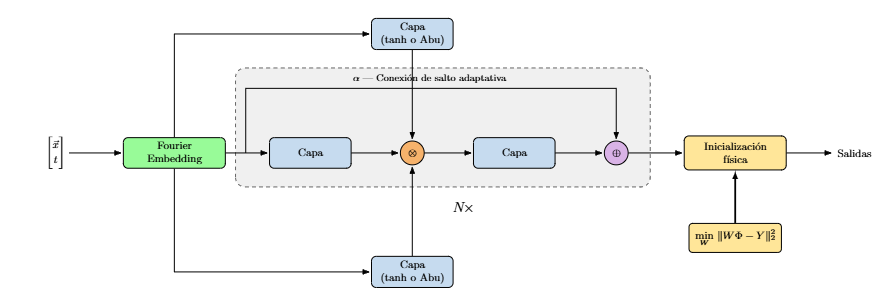
\includegraphics[width=\linewidth]{mabur_architecture.png}
  \caption[MABUR-PINN architecture]{MABUR-PINN architecture, based on PirateNet \cite{wang2024piratenets}: gates $U$ and $V$
  and the residual trunk with adaptive skip connections. Each dense block has three layers with $N$
  neurons. In Version~1 every neuron contains an Abu unit with $\{\sin,\cos,\tanh,\text{rational}\}$ and
  there is no Fourier embedding; in Version~2 the first layer of the trunk and of $U,V$ uses only $\tanh$,
  and there is a Fourier embedding.}
  \label{fig:mabur}
\end{figure}

\begin{table}[htbp]
  \centering
  \caption{The two versions of MABUR-PINN.}
  \label{tab:mabur-versions}
  \small
  \begin{tabularx}{\linewidth}{@{}lXX@{}}
    \toprule
    Property & Version 1 & Version 2 \\
    \midrule
    Implementation        & Monolithic class & Modular, four classes (modified MLP of Wang et al.~\cite{wang2021gradient}) \\
    Fourier embedding     & No & Yes, 256 random features, $\sigma=1.0$ \\
    Adaptive activation layer & AbuLayer: softmax blend of $\sin,\cos,\tanh$, rational & AbuLayer\_UV: same blend, with $U/V$ gating in a separate layer \\
    Encoders $U$ / $V$    & Adaptive layer (trainable activations) & Dense + $\tanh$ (fixed activation) \\
    Initial projection    & Adaptive layer with SIREN initialization & Dense + $\tanh$ with Glorot initialization \\
    Skip connections      & Every 3 layers & Every 2 layers \\
    $\omega_0$ (SIREN)    & 15.0 & 15.0 \\
    \bottomrule
  \end{tabularx}
\end{table}

\paragraph{Theoretical intuition.}
The Sobolev--Barron theorem (Theorem~\ref{thm:barron}) only sees the activation through the constant
$C_1=\max_{m\le\ell}\norm{\sigma^{(m)}}_{L^\infty}$. This motivates the following assumption on the family
of adaptive activations.

\begin{supuesto}{Adaptive softmax activations.}\label{asm:softmax}
Let $\Omega\subset\mathbb{R}^d$ be a bounded open domain, $\mu$ a probability measure on $\Omega$, and $\ell\in\mathbb{N}$
the maximum order of the differential operator of the PDE. Consider the family of adaptive softmax
activations
\[
  \mathcal{S}_{\mathrm{softmax}}:=\Big\{\sigma_{\mathrm{ad}}(x)=\sum_{i=1}^{N}\frac{e^{\alpha_i}}{\sum_{j=1}^{N}e^{\alpha_j}}\,\sigma_i(\beta_ix)\ \Big|\
  \bm\alpha\in\mathbb{R}^{N},\ \beta_i\in[\beta_{\min},\beta_{\max}]\subset(0,\infty)\Big\}.
\]
We assume that $\mathcal{S}_{\mathrm{softmax}}$ satisfies:
\begin{enumerate}
  \item \textbf{Uniform $C_1$ regularity:}
    $\displaystyle\sup_{\sigma_{\mathrm{ad}}\in\mathcal{S}_{\mathrm{softmax}}}\max_{m\le\ell}\norm{\sigma^{(m)}_{\mathrm{ad}}}_{L^\infty(\mathbb{R})}\le C_{1,\mathrm{ad}}<\infty.$
  \item \textbf{Sobolev--Barron approximation:} the conclusion of Theorem~\ref{thm:barron} holds for shallow
    networks whose activation is any fixed $\sigma_{\mathrm{ad}}\in\mathcal{S}_{\mathrm{softmax}}$, with
    $C_1$ replaced by $C_{1,\mathrm{ad}}$.\verificar{this condition is stated without content in the
    presentation; its validity must be checked or proved}
\end{enumerate}
\end{supuesto}

The first condition can actually be verified. Since the softmax weights $w_i$ are positive and sum to one,
by the chain rule
\begin{equation}
  \abs{\sigma^{(m)}_{\mathrm{ad}}(x)}=\Big|\sum_{i=1}^{N}w_i\beta_i^{m}\sigma_i^{(m)}(\beta_ix)\Big|
  \le\max_{1\le i\le N}\beta_{\max}^{m}\norm{\sigma_i^{(m)}}_{L^\infty(\mathbb{R})},
  \label{eq:abu-bound}
\end{equation}
so $C_{1,\mathrm{ad}}\le\max_{m\le\ell}\max_i\beta_{\max}^{m}\norm{\sigma_i^{(m)}}_{L^\infty}$, a bound that is
\emph{uniform in} $\bm\alpha$: whatever blend the optimizer learns, it can never be worse than the worst
branch at the largest scale. Two intuitions follow. First, condition~1 holds for the branches
$\{\sin,\cos,\tanh,1/(1+x^2)\}$ used for the Klein--Gordon equation (and for the Gaussian branch
$e^{-x^2}$), because they are bounded with bounded derivatives, but it fails for unbounded branches such as
Swish, Softplus or $e^{\beta x}-1$, which appear in some of the benchmark configurations
(Table~\ref{tab:benchmark-activations}). Second, the constant grows like $\beta_{\max}^{\ell}$: for the
Klein--Gordon equation ($\ell=2$) and the SIREN scale $\omega_0=15$, the factor is of order $225$. Large
scales give access to high frequencies, but they make the constant (and, by Theorem~\ref{thm:spectral-bias}, the
conditioning) worse. This is the same trade-off that $\sigma$ controls in a Fourier embedding, now learned
inside a bounded range. We stress that these are intuitions: the theorem is for shallow networks with a
single activation, while MABUR-PINN is a deep gated network whose neurons have different activations.

\paragraph{Activation functions.}
Table~\ref{tab:abu-branches} lists the candidate branches considered, with the analytical property that
justifies each of them in a PDE.

\begin{table}[htbp]
  \centering
  \caption{Candidate branches of the adaptive activation.}
  \label{tab:abu-branches}
  \small
  \begin{tabularx}{\linewidth}{@{}llX@{}}
    \toprule
    Function & Formulation $f(x)$ & Analytical property / justification in the PDE \\
    \midrule
    Sine & $\sin(\beta_ix)$ & Captures oscillatory dynamics and spatial/temporal harmonic modes. \\
    $\tanh$ & $\dfrac{e^{\beta_ix}-e^{-\beta_ix}}{e^{\beta_ix}+e^{-\beta_ix}}$ & Numerical stability; models smooth transition profiles. \\
    Swish / SiLU & $\dfrac{x}{1+e^{-\beta_ix}}$ & Good behavior of gradients in deep networks, without abrupt cancellations. \\
    Rational & $p(x)/q(x)$, e.g.\ $1/(1+(\beta_ix)^2)$ & Captures poles, asymptotes and boundary layers; high expressivity with few parameters. \\
    Exponential & $e^{\beta_ix}-1$ & Designed to capture boundary layers, strict dissipation and exponential decays. \\
    \bottomrule
  \end{tabularx}
\end{table}

\end{hyphenrules}
